\documentclass[../doc.tex]{subfiles}

\begin{document}

\section{Gameplay}

Chaque joueur se voit attribuer une cible et est cible d'un autre joueur.
Nous intégrons donc un système de sélection de cible, et un moyen pour le joueur de sélectionner un personnage (joueur ou non) à proximité de lui.

Le but est de tuer le plus de cibles joueurs dans le temps imparti.
Chaque assasinnat vous rapporte X points.

A l'aide de de classe de personnage, nos personnages \textbf{pourraient} avoir des pouvoirs spécifiques,
tel que se déguiser en quelqu'un d'autre pendant une durée limitée,
pouvoir tuer à moyenne distance, ralentir et afaiblir un joueur
(l'empêcher de courir, d'utiliser des capacités par exemple), avoir une boussole plus précise\dots


Nous avons également rajouté des objets pouvant être utilisé par les joueurs
(Echelles\footnote{Voir Figure 4}, Portes) et comptons en rajouter d'autres.
\begin{figure}[hbt!]
    \centering
    \begin{subfigure}[t]{0.3\textwidth}
        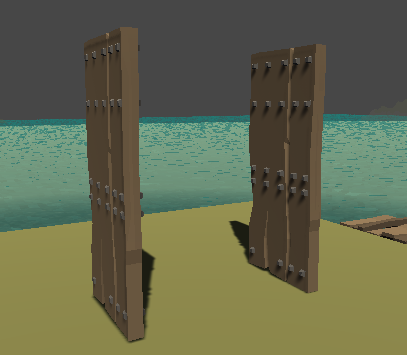
\includegraphics[scale=0.5]{doors_open.png} 
        \caption{Portes ouvertes}
    \end{subfigure}
    \hspace{50pt}
    \begin{subfigure}[t]{0.3\textwidth}
        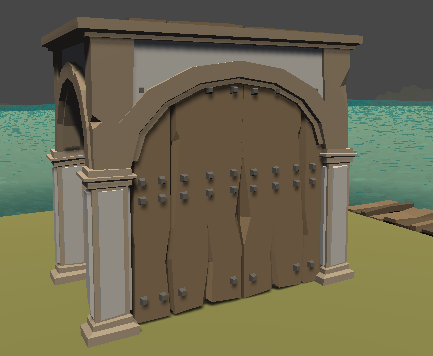
\includegraphics[scale=0.5]{doors_closed.png}
        \caption{Portes fermée avec arche}
    \end{subfigure}
    \caption{Exemple des portes que nous avons réalisé}
\end{figure}

\end{document}